\section{Diagonalisierung}
\subsection[Einleitung]{Einleitung}
\begin{frame}
	\frametitle{Einleitung}
	\framesubtitle{Diagonalisierung : Was ist das eigentlich?}
	
	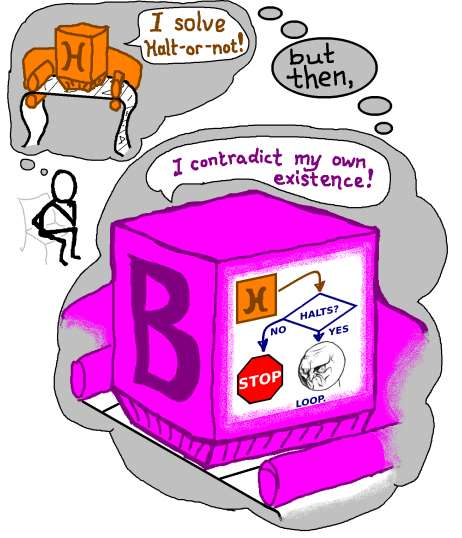
\includegraphics[scale = 0.3]{halting-problem.jpg}
\end{frame}
\begin{frame}
	\frametitle{Einleitung}
	\framesubtitle{Eine Hierarchie von Komplexitätsklassen}
	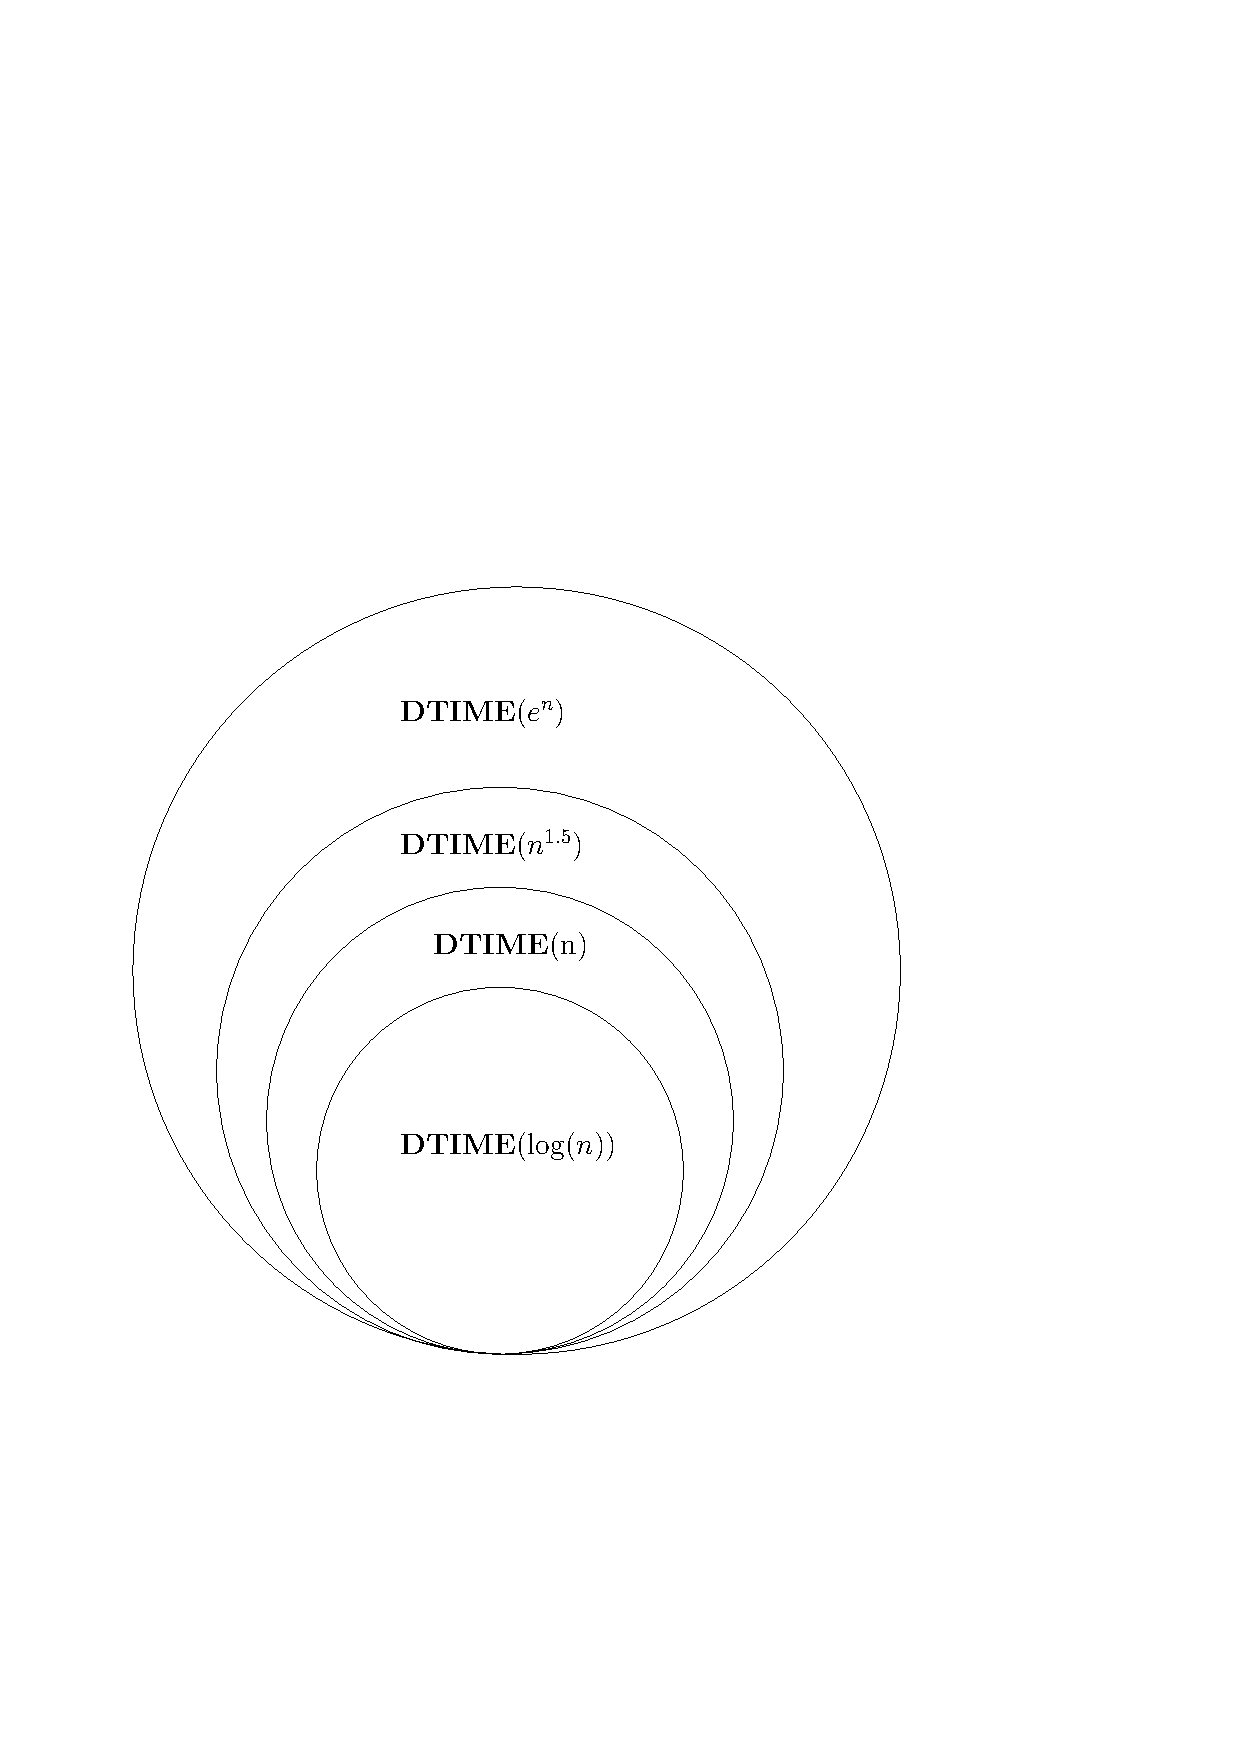
\includegraphics[scale=0.5]{images/timehierarchy.pdf}
\end{frame}
\begin{frame}
	\frametitle{Einleitung}
	\framesubtitle{$\P$ oder $\NPC$ : gibt es noch mehr in $\NP$?}
	\overprint{
		\only<1>{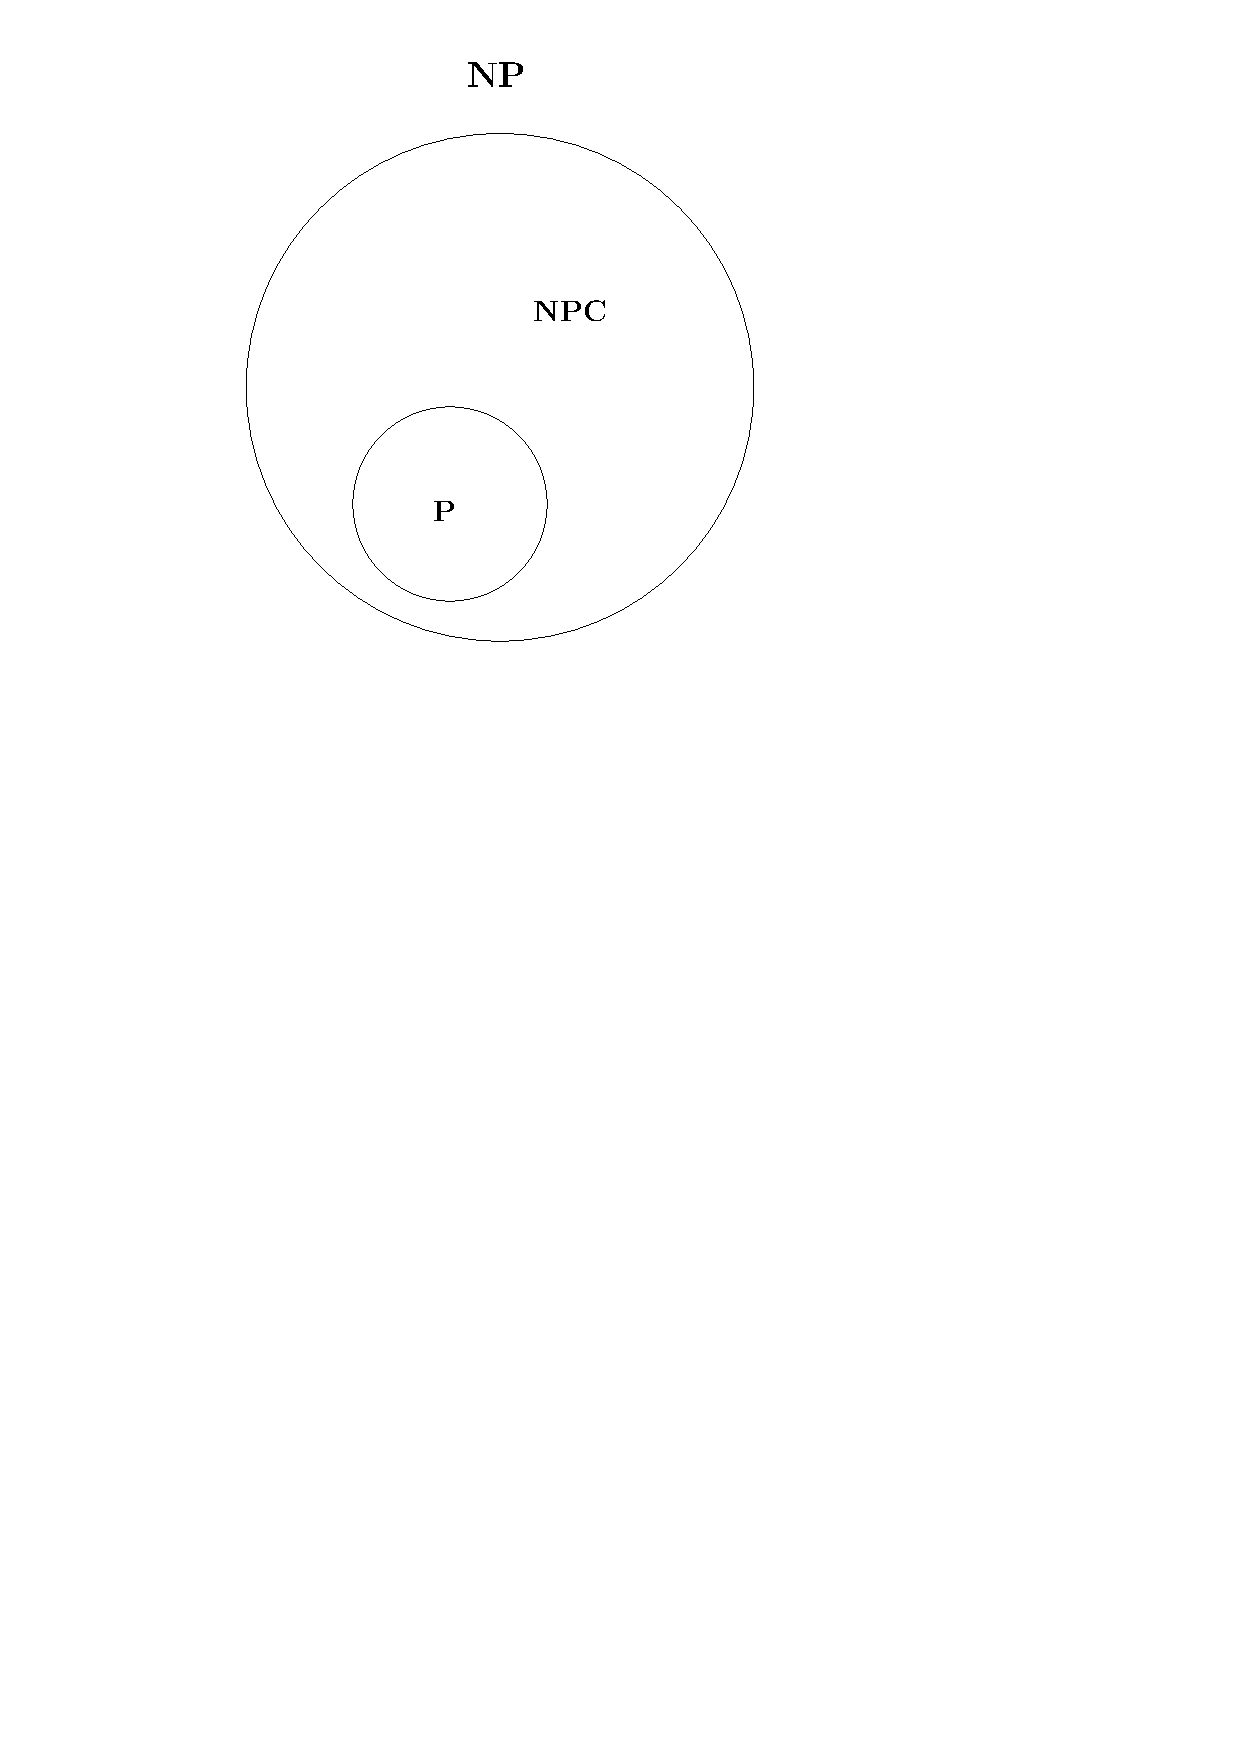
\includegraphics[page = 1,scale = 0.6]{images/npi.pdf}}
		\only<2>{\includegraphics[page = 2,scale = 0.6]{images/npi.pdf}}
	}
\end{frame}
\begin{frame}
	\frametitle{Einleitung}
	\framesubtitle{Grenzen der Diagonalisierung}
	
	\begin{itemize}[<+->]
	  \item Orakelmaschinen und die P, NP Frage
	  \item Polynomial Hierarchy : Eine Verallgemeinerung von \P , \NP
	\end{itemize}
\end{frame}

\begin{frame}{Gliederung}
  \tableofcontents
\end{frame}
\subsection[Diagonalisierung]{Was verstehen wir unter Diagonalisierung?}
\begin{frame}
	\frametitle{Diagonalisierung}
	\framesubtitle{Was verstehen wir darunter?}
	
	
	


	\begin{figure}
			\begin{minipage}{0.8\linewidth}
				\begin{itemize}[<+->]
					\item Cantors Diagonalargument zur Überabzählbarkeit von $ \mathbb{R}$
					\item Unentscheidbarkeit des Halteproblems
					\item informell: Konstruktion eines Elements, das sich von jedem anderen Element unterscheidet
					\item Diagonalisierung nicht immer "schön" zu sehen
				\end{itemize}
			\end{minipage}
			\begin{minipage}{0.1\linewidth}
					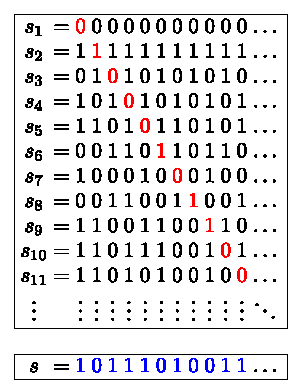
\includegraphics[scale = 0.4]{images/Diagonal_argument_svg.pdf}%
			\end{minipage}
		\end{figure}
	
\end{frame}
\begin{frame}
	\frametitle{Diagonalisierung}
	\framesubtitle{Was verstehen wir darunter?}
	\begin{KITinfoblock}{Was ist Diagonalisierung} {
			Als Diagonalisierung wird (hier) ein Beweis bezeichnet, der nur auf den beiden folgenden
			Eigenschaften von TM aufbaut.
			
			\begin{enumerate}
				\item<2-> Die Existenz einer Repräsentation von TM durch Zeichenketten (Gödelnummer)
				\item<3-> Die Fähigkeit eine andere TM mit geringem zusätzlichen Zeit- oder Platzbedarf zu simulieren (Universelle TM)
			\end{enumerate}		
		}
	\end{KITinfoblock}
	
\end{frame}
\subsection[Time Hierarchy]{Time Hierarchy}
\begin{frame}
	\frametitle{Time Hierarchy}
	\framesubtitle{Vorraussetzungen}
	Wiederholung :
	\begin{itemize}[<+->]
		\item Für $i\in \mathbb{N}$ beschreibt i die TM $M_i$
		\item Jede TM wird von unendlich vielen $i\in \mathbb{N}$ beschrieben
		\item Es existiert eine universelle TM U, die jede TM mit logarithmischem Overhead 					simulieren kann
	\end{itemize}
\end{frame}
\begin{frame}
	\frametitle{Time Hierarchy}
	\framesubtitle{Vorraussetzungen}
	\begin{KITexampleblock}{Universelle TM}
	TM $M_i$ läuft bei Eingabe x in $\mathcal{O}(f(n))$
	$\Rightarrow$ TM U läuft bei Eingabe i, x in $\mathcal{O}(f(n)log(fn))$
	\end{KITexampleblock}
\end{frame}
\begin{frame}
	\frametitle{Time Hierarchy}
	\framesubtitle{Vorraussetzungen}
	\begin{KITinfoblock}{Definition Time-constructible functions}
		Wir nennen eine Funktion f time-constructible, falls gilt : \newline
		f(n) ist in $\mathcal{O}(f(n))$ berechenbar. 
	\end{KITinfoblock}
	
	\bigskip
	\pause	
	
	\begin{KITinfoblock}{Definition \DTIME }
		\DTIME(f(n)) = $\lbrace$ L $\vert \exists$ deterministische Turingmaschine ,
		 die L in $\mathcal{O}(f(n))$ entscheidet $\rbrace$
	\end{KITinfoblock}
\end{frame}
\begin{frame}
	\frametitle{Time Hierarchy}
	\framesubtitle{Deterministische Time Hierarchy}
	
	\begin{KITinfoblock}{Satz Time Hierarchy Theorem, 65}
	Wenn f, g  time-constructible Funktionen sind die  
	$f(n)\log(f(n)) \in o(g(n))$ erfüllen, dann gilt

		$\DTIME(f(n)) \subsetneq \DTIME(g(n))$
		
	\end{KITinfoblock}
	
	\pause

	Frage : Warum brauchen wir den Faktor $\log(f(n))$ ?
\end{frame}

\begin{frame}
	\frametitle{Time Hierarchy}
	\framesubtitle{Deterministische Time Hierarchy}
	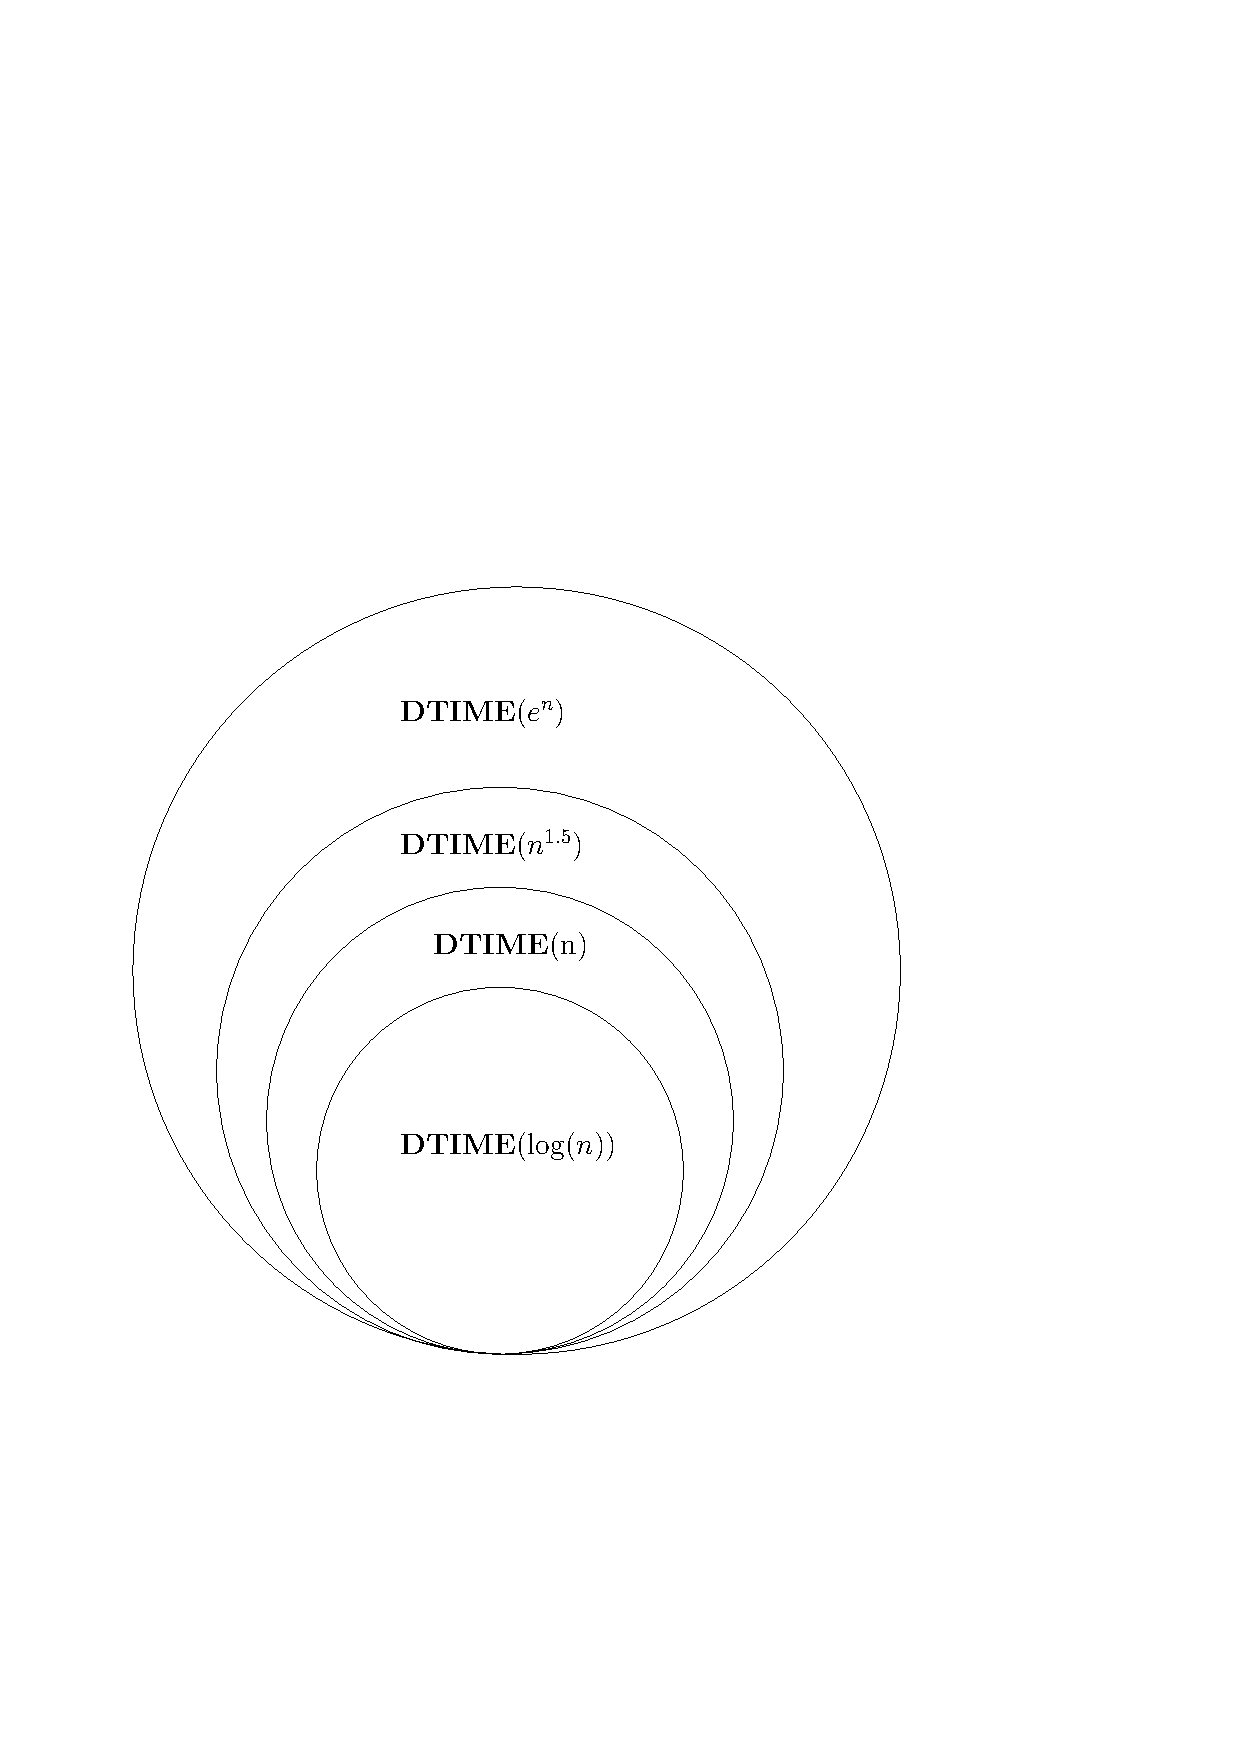
\includegraphics[scale=0.5]{images/timehierarchy.pdf}
\end{frame}

\begin{frame}
	\frametitle{Time Hierarchy}
	\framesubtitle{{Beweis det. Time Hierarchy}}
	Wir zeigen nur $\DTIME(n) \subsetneq \DTIME(n^{1.5})$
	\bigskip
	\pause
	\begin{KITblock}{Definition Turing Maschine D} 
		Bei Eingabe x : Simuliere die TM $M_x$ mit Eingabe x genau für $|x|^{1.4}$ 						Schritte. Danach gebe folgendes aus :
		\begin{equation}
		D(x) = 
		\begin{cases}
			\overline{M_x(x)} & \text{falls die Simulation eine Ausgabe hatte} \\
			0 & \text{sonst}
			
		\end{cases}
		\end{equation}			
	\end{KITblock}
	\bigskip
	\pause	
	
	\begin{KITblock}{Die von D erzeugte Sprache}
		Sei L = $ \lbrace x \vert D(x) = 1  \rbrace$
	\end{KITblock}
\end{frame}

\begin{frame}
	\frametitle{Time Hierarchy}
	\framesubtitle{Beweis det. Time Hierarchy}
	\begin{KITblock}{Behauptung}
		$L \in \DTIME(n^{1.5})$ und $L \notin \DTIME(n)$
	\end{KITblock}
	\pause
	\begin{itemize}[<+->]
		\item Wir nehmen an , dass $L \in \DTIME(n)$
		\item $\Rightarrow \exists$ Turing Maschine M , die L entscheidet und für Eingabe x
		 		höchstens c|x| Schritte benötigt. (c ist konstant)
		\item $\Leftrightarrow \forall x \in {\lbrace 0,1 \rbrace }^{*}$ D(x) = M(x)
	\end{itemize}
\end{frame}

\begin{frame}
	\frametitle{Time Hierarchy}
	\framesubtitle{Beweis det. Time Hierarchy}
	\begin{itemize}[<+->]
		\item Wollen nun M auf D simulieren können
		\item M simuliert auf U läuft in $c|x|\log(|x|)$
		\item Wir wählen dazu $n_0$ so groß, dass $\forall$ $n \geq n_0$ gilt :
			$n^{1.4} > cn\log(n)$		
		\item Nun wählen wir eine Gödelnummer x , so dass $|x| > n_0$ und $M_x$ = M
		\item Nun gilt $D(x) \neq M(x)$ 
		
		\qed 
	\end{itemize}
\end{frame}

\subsection[Satz von Ladner]{Satz von Ladner}
\begin{frame}
	\frametitle{Satz von Ladner}
	\framesubtitle{Motivation}
	\includegraphics[page = 2,scale = 0.6]{images/npi.pdf}
	Frage : Gibt es $\NP$  Probleme, die nicht \NP -vollständig sind, aber auch
	nicht in $\P$  liegen?
\end{frame}
\begin{frame}
	\frametitle{Satz von Ladner}
	\framesubtitle{\NP -intermediate Probleme}
	Mögliche Kandidaten :
	\begin{itemize}
	\item Graphisomorphie (kommt in Vortrag 7)
	\item Faktorisierungsproblem
	\item Kein "natürliches" Problem bekannt
	\end{itemize}
	
	aber,
\end{frame}

\begin{frame}
	\frametitle{Satz von Ladner}
	\framesubtitle{Behauptung}
	\begin{KITinfoblock}{Existenz einer \NP -intermediate Sprache, Ladner, 75}
	Wenn $\P \neq \NP$ dann gilt : \newline
	Es existiert eine Sprache $L \in \NP \setminus \P$ die nicht \NP -vollständig ist
	\end{KITinfoblock}
\end{frame}
\begin{frame}
	\frametitle{Satz von Ladner}
	\framesubtitle{Beweisidee}
	Konstruieren Sprache mit diesen Eigenschaften und zeigen, dass sie in $\NP$ -
	intermediate ist, falls $\P \neq \NP$  :
	
	\bigskip
	\pause
	\begin{KITinfoblock}{Die Sprache ${\SAT}_H$}
		Für eine Funktion $H$ : $\mathbb{N} \rightarrow \mathbb{N}$ definieren wir : \newline 	
		${\SAT}_H = \lbrace \psi 01^{n^{H(n)}} : \psi \in \SAT$ und $ n = |\psi| \rbrace$
	\end{KITinfoblock}
	\bigskip
	\pause	
	
	\begin{KITexampleblock}{Beispiel für ${\SAT}_H$}
	F\"ur $H(n) = n - 1$ und $\psi = a \land b$ gilt : \newline
	$(a \land b) 01^{3^2} = (a \land b) 0111111111 \in {\SAT}_H $
	\end{KITexampleblock}
\end{frame}

\begin{frame}
	\frametitle{Satz von Ladner}
	\framesubtitle{Beweis : Wahl von $H$}
	\begin{KITinfoblock}{Definition von $H$}
		\begin{itemize}
		\item Betrachte die TM $M_1, M_2, ..., M_{\lfloor \log(\log(n)) \rfloor}$. \newline
		\item Wähle unter diesen die TM $M_i$ mit kleinster Gödelnummer $i$, welche für alle
		$|x| \leq \log(n) $  ${\SAT}_H(x)$
		in $i|x|^i$ Schritten berechnet
		\item Setze $H(n) = i$. 
		\item Falls eine solche TM nicht existiert, setze $H(n) = \log(\log(n))$
		\end{itemize}
	\end{KITinfoblock}
	\pause
	\begin{KITblock}{Gewähltes $H$ erfüllt die folgenden Eigenschaften}
		${\SAT}_H \in \P \Leftrightarrow H(n) \in O(1)$ (also $H(n) \leq C$ f\"ur alle n) 				\newline
		und damit insbesondere $\lim_{n \to \infty}  H(n) = \infty$ f\"ur ${\SAT}_H
		\notin \P$
	\end{KITblock}
	\pause
	\begin{itemize}
	  \item  $H$ erfüllt diese und ist polynomiell berechenbar.
	  \item (ohne Beweis)
	\end{itemize}
		
\end{frame}
% \begin{frame}{Beweis von Ladner}
% 	\framesubtitle{Nachweis der Eigenschaften von H}
%  	\begin{KITinfoblock}{Definition von H}
% 		$H(n)$ ist die kleinste Gödelnummer $i < \log (\log (n))$ so dass für alle
% 		$ x \in \{0,1\}^*$ mit $|x| \leq \log(n) $ die Turing Maschine $M_i$ genau ${\SAT}_H(x)$
% 		in $i|x|^i$ Schritten berechnet. Falls dieses $i$ nicht existiert setzen wir 
% 		$H(n) = \log(\log(n))$ 
% 	\end{KITinfoblock}
% 	\pause
% 	
% 	\begin{overprint}
% 		\only<2-5> {
% 			\bigskip
% 		Zuerst zeigen wir : ${\SAT}_H \in \P \Rightarrow H(n) \in O(1)$
% 		\pause
% 		\begin{itemize}[<+->]
% 			\item ${\SAT}_H \in \P \Rightarrow \exists$ Turing Maschine $M$, die
% 			${\SAT}_H$ in höchstens $cn^c$ Schritten entscheidet.
% 			\item $\exists i > c$ , so dass $M_i$ = M
% 			\item Für n > $2^{2^i}$ gilt $H(n) \leq i$ und damit $H(n) \in O(1)$ 
% 		\end{itemize}
% 		}
% 		\only<6-> {
% 			\bigskip
% 			Nun : $ H(n) \in \mathcal{O}(1) \Rightarrow {\SAT}_H \in \P$
% 			\pause
% 			\begin{itemize}
% 				\item<7-> Da $ H(n) \in \mathcal{O}(1)$ ist Bild von $H$ endlich $ \Rightarrow \exists i$ mit $H(n) = i$ für unendlich viele $n$
% 				\item<8-> TM $M_i$ löst ${SAT}_H$ in $ in^i$ Schritten
% 				\item<9-> Denn, angenommen $\exists x$ für welches $M_i$ dies nicht in dieser Grenze schafft $\Rightarrow$ $H(n) \neq i$ für alle $ n > 2^{|x|} $
% 				nach Definition von $H$
% 				
% 			\end{itemize}
% 		
% 		}
% 	\end{overprint}
% 	
% 	
% \end{frame}
\begin{frame}{Beweis von Ladner}
	\framesubtitle{${\SAT}_H$ weder in $\P$ noch  $\NP$-complete}
	\begin{KITinfoblock}{Definition von ${\SAT}_H$} 	
		${\SAT}_H = \lbrace \psi 01^{n^{H(n)}} : \psi \in \SAT$ und $ n = |\psi| \rbrace$
	\end{KITinfoblock}
	\begin{KITblock}{Gewähltes $H$ erfüllt die folgenden Eigenschaften}
			${\SAT}_H \in \P \Leftrightarrow H(n) \in O(1)$ (also $H(n) \leq C$ f\"ur alle n) 		
	\end{KITblock}
	\pause
	\bigskip
	\heading{${\SAT}_H$ ist nicht in $\P$}
	\pause
	\bigskip
	\begin{itemize}[<+->]
		\item Angenommen ${\SAT}_H \in \P \Rightarrow $  $H(n) \le C$, $C$ Konstante
		\item ${\SAT}_H$ ist also $\SAT$  mit höchsten polynomiell vielen  angehängten 1en
		\item $\SAT$ kann somit durch dieselbe TM wie ${\SAT}_H$ gelöst werden
			\begin{itemize}
				\item Konstruiere für Eingabe $\varphi$ die ${\SAT}_H$-Instanz $\varphi01^{|\varphi|^{H_(|\varphi|)}}$ 
				\item gebe diese Instanz in TM, welche ${\SAT}_H$ polynomiell entscheidet
			\end{itemize}
			\item $\Rightarrow \P = \NP$
	\end{itemize}
	
\end{frame}

\begin{frame}{Beweis von Ladner}
		\framesubtitle{${\SAT}_H$ weder in $\P$ noch $\NP$-complete}
	
		\begin{KITinfoblock}{Definition von ${\SAT}_H$}	
			${\SAT}_H = \lbrace \psi 01^{n^{H(n)}} : \psi \in \SAT$ und $ n = |\psi| \rbrace$
		\end{KITinfoblock}
		
		
		\bigskip
		\only<2->{\heading{${\SAT}_H$ ist nicht in $\NPC$}}
		\pause
		\bigskip
		
		\begin{itemize}[<+->]
			\item Angenommen ${\SAT}_H \in \NPC \Rightarrow $ es existiert poly. Reduktion $f$ von $\SAT$ auf ${\SAT}_H$.
			\item Da ${\SAT}_H \notin \P $ geht $H(n)$ gegen $\infty$ 
			\item $\SAT$-Instanz $\varphi$ wird mit $f$ auf ${\SAT}_H$-Instanz der Form $\psi01^{{\psi}^{H(|\psi|)}}$ abgebildet.
			\item $|f(\varphi)|=|\psi| + |0| + {|\psi|}^{H(|\psi|)}$
		\end{itemize}
\end{frame}
\begin{frame}{Beweis von Ladner}
	\framesubtitle{${\SAT}_H$ weder in $\P$ noch $\NP$-complete}
	
	\begin{KITinfoblock}{Definition von ${\SAT}_H$}	
		${\SAT}_H = \lbrace \psi 01^{n^{H(n)}} : \psi \in \SAT$ und $ n = |\psi| \rbrace$
	\end{KITinfoblock}
		\begin{itemize}[<+->]
		\item Für beliebig große $\SAT$-Instanz $\varphi$ wird $|\psi|$ in ${\SAT}_H$ beliebig groß.
		\item $\Rightarrow$ ab gewisser Größe müssen $\SAT$-Instanz $\varphi$ von $f$ auf ${\SAT}_H$-Instanz mit $|\psi| \in o(n)$  abgebildet werden.
		 
		\item Ansonsten wegen $H(n)$ gegen $\infty$ \newline $|{|\psi|}^{H(|\psi|)}|$  und damit $ \Rightarrow|\psi01^{|\psi|^{H(|\psi|)}} |$  größer als jedes $p(|\varphi|)$.
		\item $|\psi|$ also echt kleiner als $\frac{|\varphi|}{2}$
		\item Algorithmus der $\SAT$ in poly. Zeit entscheidet 
			\begin{itemize}
				\item bilde $\SAT$-Instanz $\varphi$ mit $f$ auf $\psi01^{|\psi|^{H(|\psi|)}}$ ab
				\item $|\psi|$ kleiner $\frac{|\varphi|}{2}$ und es gilt $\varphi \in \SAT \Leftrightarrow \psi \in \SAT$ 
				\item Wiederhole ersten Schritt mit $\psi$ als Eingabe
			\end{itemize}
		\item Widerspruch zu $\P \neq \NP$
		\end{itemize}
\end{frame}
\subsection[Orakelmaschinen]{Orakelmaschinen - Grenzen der Diagonalisierung}

\begin{frame}
	\frametitle{Grenzen der Diagonalisierung}
	\framesubtitle{Wiederholung Diagonalisierung}
	\begin{KITinfoblock}{Was ist Diagonalisierung} {
			Als Diagonalisierung wird (hier) ein Beweis bezeichnet, der nur auf den beiden folgenden
			Eigenschaften von TM aufbaut.
			
			\begin{enumerate}
				\item<2-> Die Existenz einer Repräsentation von TM durch Zeichenketten (Gödelnummer)
				\item<3-> Die Fähigkeit eine andere TM mit geringem zusätzlichen Zeit- oder Platzbedarf zu simulieren (Universelle TM)
			\end{enumerate}		
		}
	\end{KITinfoblock}
\end{frame}

\begin{frame}
	\frametitle{Grenzen der Diagonalisierung}
	\framesubtitle{Definition von Orakelmschinen}
	\begin{itemize}
		\item Werden zeigen, dass Diagonalisierung allein $\P/\NP$ Frage nicht beantworten kann
		\item benötigen hierzu ein weitere Kategorie von Turingmaschinen. 
	\end{itemize}
	\begin{KITinfoblock}{Definition Orakel-Turingmaschine} {
			Eine Orakel-Turingmaschine $M$ ist eine TM, die folgende zusätzliche Eigenschaften hat:
			\begin{itemize}
				\item<2-> ein spezielles zusätzliches Band (Orakelband) und 3 spezielle zusätzliche Zustände $q_{query}, q_{yes}, q_{no}$.
				\item <3-> ein Orakel $O \subseteq \{0,1\}^*$
				\item <4-> Wenn $M$ den Zustand $q_{query}$ betritt, ist der Folgezustand
					\begin{itemize}
					\item $q_{yes}$, wenn für Inhalt $s$ des Orakelbands gilt $s \in O$ und
				    \item	$q_{no}$, wenn  $s \notin O$ 
					\end{itemize} 
				\item<5-> Das Orakel liefert die Antwort \alert{in einem Berechnungsschritt}
			\end{itemize}
		}
	\end{KITinfoblock}
\end{frame}
\begin{frame} 
	\frametitle{Grenzen der Diagonalisierung}
	\framesubtitle{Satz von Baker-Gill-Solovay}
	\begin{KITinfoblock}{Komplexitätsklassen von Orakelmaschinen}
		Für jedes $\mathbf{O} \subseteq \{0,1\}^*$ ist ${\P}^{\mathbf{O}}$ die Menge
		aller Sprachen, die eine det. Orakel-TM mit Orakel $\mathbf{O}$ entscheiden
		kann.
		${\NP}^{\mathbf{O}}$ analog für nichtdet. Orakel-TM.
		
	\end{KITinfoblock}
	\bigskip
	\pause
	\begin{KITinfoblock}{Satz (Baker,Gill,Solovay, 75)}
		Es existieren Orakel A, B so dass ${\P}^A = {\NP}^A$ und ${\P}^B \neq {\NP}^B$
	\end{KITinfoblock}
\end{frame}
\begin{frame}
	\frametitle{Grenzen der Diagonalisierung}
	\framesubtitle{relativierende Beweise}
	\begin{KITinfoblock}{Satz (Baker,Gill,Solovay, 75)}
		Es existieren Orakel A, B so dass ${\P}^A = {\NP}^A$ und ${\P}^B \neq {\NP}^B$
	\end{KITinfoblock}
	\bigskip
	\begin{overprint}
		\only<1-2>{
		
		\begin{KITinfoblock}{relativierende Beweise}
			Wir nennen einen Beweis, der auch für TM mit Orakel gilt, einen \newline
			\emph{relativierenden Beweis}
		\end{KITinfoblock}
		\begin{itemize}[<+->]
		\item Diagonalisierung ist relativierend und kann damit nicht f\"ur die $\P
		- \NP$ Frage genutzt werden.
		\item $\Rightarrow$ ein Beweis für die $\P-\NP$ Frage muss ein nicht
		relativierendes Verfahren nutzen !
		\end{itemize}
		}
		
	\end{overprint}
\end{frame}

\begin{frame}
	\frametitle{Grenzen der Diagonalisierung}
	\framesubtitle{Beispiele für Orakelmaschinen}
	\heading{$\overline{\SAT}$}
	\begin{itemize}[<+->]
		\item   Für $\overline{\SAT}$, Sprache der nicht erfüllbaren Formeln, gilt
		$\overline{SAT} \in {\P}^{\SAT}$.
		\item   Mit  Orakel $\SAT$ kann TM in $\mathcal{O}(1)$ entscheiden, ob
		$\varphi \in \SAT$ und gegenteilige Antwort ausgeben.
	\end{itemize}
\end{frame}

\begin{frame}
	\frametitle{Grenzen der Diagonalisierung}
	\framesubtitle{Beweis : ${\P}^A = {\NP}^A$ }
	\heading{Beweis des Satzes von Baker:} 
	\begin{itemize} [<+->]
		\item Sei $\mathbf{EXPCOM}$ folgende Sprache: \[\{(M,x,1^n) : M \  entscheidet \ x \ innerhalb \ von \ 2^n \ Schritten  \}
		 \] 
			Dann gilt ${\P}^{\mathbf{EXPCOM}} = {\NP}^{\mathbf{EXPCOM}} = \EXP$.
			\item $ \EXP \subseteq {\P}^{\mathbf{EXPCOM}} $
			\begin{itemize}
				\item TM $M$ entscheidet $L \in \EXP$
				\item Baue Orakel-TM, die Orakel mit $(M,x,|x|)$ aufruft
			\end{itemize}
			\item ${\NP}^{\mathbf{EXPCOM}} \subseteq \EXP$
			\begin{itemize}
				\item  $M$  nichtdet. TM mit Orakel $\mathbf{EXPCOM}$: 
				\item Ausführung von $M$ det. in Exponentialzeit simulieren
				\item Orakelaufruf in Exponentialzeit simulieren (max $2^{|x|} \cdot 2^{q(|x|)}$ Schritte)	
			\end{itemize}
			
			
			\item $\Rightarrow \EXP \subseteq{\P}^{\mathbf{EXPCOM}} \subseteq {\NP}^{\mathbf{EXPCOM}} \subseteq \EXP$ 
			
	\end{itemize}
\end{frame}

\begin{frame}
	\frametitle{Grenzen der Diagonalisierung}
	\framesubtitle{Beweis : ${\P}^B \neq {\NP}^B$}
	\begin{KITinfoblock}{Definition unäre Sprache $U_B$}
		Für eine Sprache B sei $U_B = \lbrace 1^n :$ Es gibt einen String
		der L\"ange n in B $\rbrace $
	\end{KITinfoblock}	
	\pause
	
	\begin{itemize}[<+->]
		\item Warum gilt $U_B \in {\NP}^B$?
		\item M\"ussen also nur noch B so konstruieren, dass $U_B \notin {\P}^B$
	\end{itemize}
\end{frame}

\begin{frame}
	\frametitle{Grenzen der Diagonalisierung}
	\framesubtitle{Konstruktion von B}
	Wir konstruieren eine Folge von Sprachen $(B_i)_{i \in \mathbb{N}}$ so , dass 
	$B = \lim_{i \to \infty} B_i$	
	\begin{itemize}[<+->]
		\item Wie stellen wir sicher, dass keine Turing Maschine $U_B$
			in polynomieller Zeit entscheiden kann?
		\item Tipp: Die Menge aller Turing Maschinen ist abzählbar
	\end{itemize}
\end{frame}

\begin{frame}
	\frametitle{Grenzen der Diagonalisierung}
	\framesubtitle{Konstruktion von B}
	\begin{itemize}[<+->]
	\item Genau : Wir iterieren über alle Turing Maschinen $M_i$ und stellen
	sicher, dass $M_i$ nicht in polynomieller Zeit $U_B$ entscheiden kann
	\item Nutze dabei, dass die Anzahl der Wörter exponentiell in der Eingabelänge wächst
	\end{itemize}
\end{frame}

\begin{frame}
	\frametitle{Grenzen der Diagonalisierung}
	\framesubtitle{Konstruktion von B}
	Wir fangen an mit $B_0 = \emptyset$. Konstruktion f\"r $B_i$ :
	\begin{itemize}[<+->]
		\item Wähle n so , dass n größer als alle Strings in $B_{i-1}$
		\item Lasse $M_i$ auf Eingabe $1^n$ genau $2^n / 10$ Schritte laufen \newline
			(Beachte, dass $M_i$ das Orakel B hat!)
	\end{itemize}
\end{frame}
\begin{frame}
	\frametitle{Grenzen der Diagonalisierung}
	\framesubtitle{Konstruktion von B}
	\begin{columns}
	\column{.5\textwidth}
	
	\only<1>{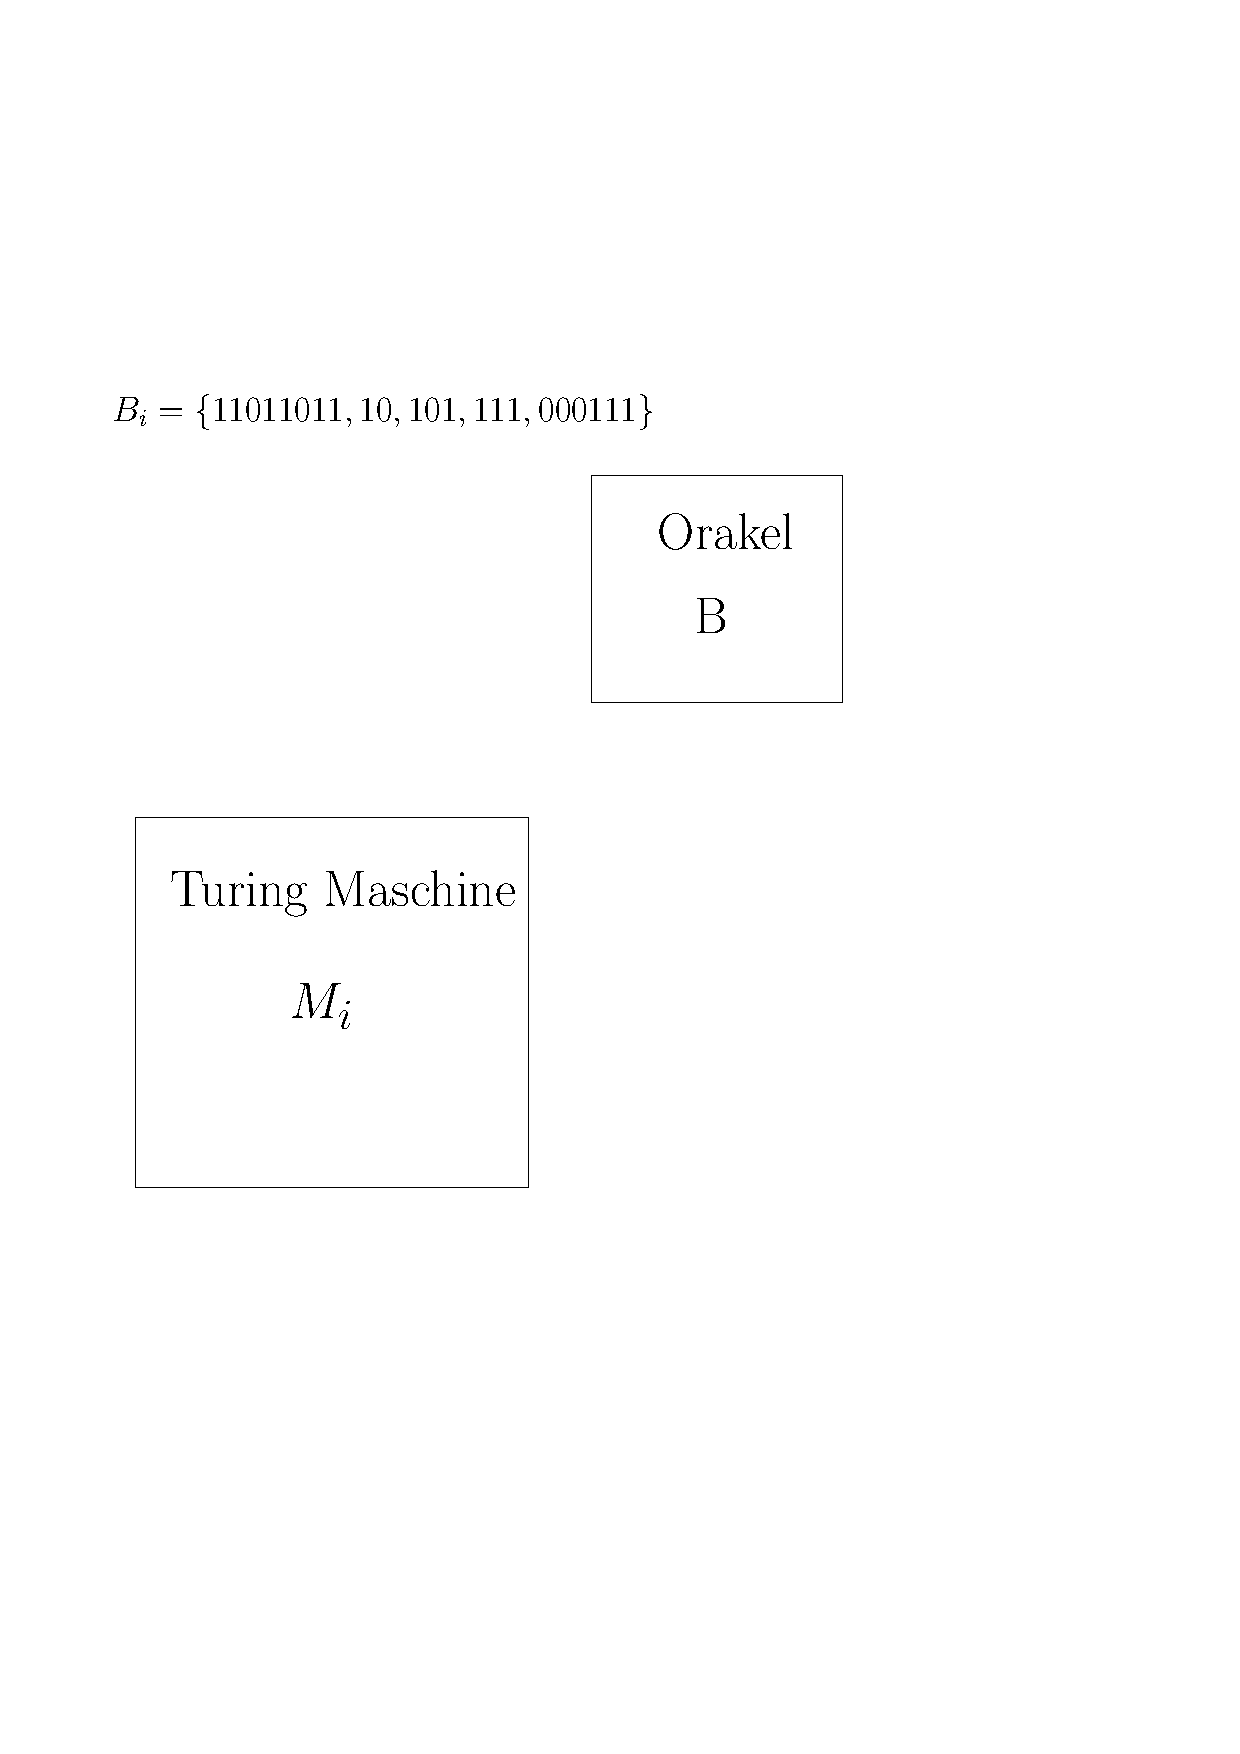
\includegraphics[page=1, scale= 0.5]{images/b_construction.pdf}}
	\only<2>{\includegraphics[page=2, scale= 0.5]{images/b_construction.pdf}}
	\only<3>{\includegraphics[page=3, scale= 0.5]{images/b_construction.pdf}}
	\only<4>{\includegraphics[page=4, scale= 0.5]{images/b_construction.pdf}}
	\only<5>{\includegraphics[page=5, scale= 0.5]{images/b_construction.pdf}}
	\only<6>{\includegraphics[page=6, scale= 0.5]{images/b_construction.pdf}}
	
	\column{.5\textwidth}
	\begin{itemize}
	  \item Das Orakel antwortet konsistent auf dem bisherigen $B_i$
	  \item Wir merken uns alle Strings der L\"ange n, die $M_i$ an fragt!
	\end{itemize}
	\end{columns}
\end{frame}

\begin{frame}
	\frametitle{Grenzen der Diagonalisierung}
	\framesubtitle{Konstruktion von B}
	\begin{itemize}[<+->]
	  \item Wir definieren nun $B_{i+1}$ wie folgt :
	  \item Wenn $M_i$ nicht gehalten hat : $B_{i+1} = B_i$
	  \item ansonsten : \begin{itemize}
	    \item $M_i$ akzeptiert $1^n$ : Wir definieren, dass kein String der Länge n
	    in B ist
	    \item $M_i$ lehnt ab : Wähle $x \in {\lbrace 0,1 \rbrace}^n$, welches nicht
	    von $M_i$ an gefragt wurde und setze $B_{i+1} = B_i \cup \lbrace x \rbrace$
	    \item warum existiert dieses x?
	    \end{itemize}
	\end{itemize}
\end{frame}

\begin{frame}
	\frametitle{Grenzen der Diagonalisierung}
	\framesubtitle{Beweis Schluss}
	
	\begin{itemize}[<+->]
	  \item Haben oben ein gesehen, dass $U_B \in {\NP}^B$
	  \item Und f\"ur jede polynomiell beschränkte TM M existiert ein i,so dass 
	  	\begin{itemize}
	  	  \item M = $M_i$
	  	  \item M auf der Eingabe $1^i$ weniger als $2^i / 10 $ Schritte benötigt
	  	  \item und damit $M_i$ nach Konstruktion die Frage $1^i \in U_B$ falsch
	  	  beantwortet
	  	 \end{itemize}
	  	\item $\Rightarrow U_B \notin {\P}^B$ und damit ${P}^B \neq {\NP}^B$ \qed
	\end{itemize}
\end{frame}